\documentclass[11pt]{extarticle}
\usepackage{manualdoprofessor}
\usepackage{fichatecnica}
\usepackage{lipsum,media9}
\usepackage[justification=raggedright]{caption}
\usepackage[one]{bncc}
\usepackage[lunna]{../edlab}
\usepackage{marginnote}
\usepackage{pdfpages}
\usepackage[printwatermark]{xwatermark}
\newwatermark[pagex=2]{
\includegraphics[scale=3.3]{watermarks/test-a.png}}  % página específica
%\newwatermark[oddpages]{
\includegraphics{watermarks/test-a.png}}           % páginas ímpars
%\newwatermark[evenpages]{
\includegraphics{watermarks/test-a.png}}          % págimas pares
\newwatermark[allpages]{
\includegraphics[scale=3.3]{watermarks/test-b.png}}

\pagecolor{cyan!0!magenta!10!yellow!28!black!28!}

\newcommand{\AutorLivro}{Lucas-K}
\newcommand{\TituloLivro}{Almanaque de bichos}
\newcommand{\Tema}{Animais da fauna local; nacional e mundial}
\newcommand{\Genero}{Prescritivos: instruções; guias; manuais; ciclo de crescimento; ciclo de vida etc}
%\newcommand{\imagemCapa}{./images/PNLD0001-01.png}
\newcommand{\issnppub}{978-65-99441-25-7}
\newcommand{\issnepub}{978-65-99441-26-4}
% \newcommand{\fichacatalografica}{PNLD0001-00.png}
\newcommand{\colaborador}{{Paulo Pompermaier e Renier Silva}}

\begin{document}

\title{\TituloLivro}
\author{\AutorLivro}
\def\authornotes{\colaborador}

\date{}
\maketitle

%\begin{abstract}\addcontentsline{toc}{section}{Carta ao professor}
%\pagebreak

\tableofcontents



\section{Sobre o livro}

%27 caracteres
\paragraph{O livro} 
``Almanaque de bichos'' é um livro composto por palavras e ilustrações. 

%822 caracteres
\paragraph{Descrição} 
Com o objetivo de apresentar às crianças as letras do alfabeto da língua portuguesa,
a cada palavra elas conhecerão um animal cuja inicial corresponda à letra em ordem alfabética.
São privilegidos animais da fauna nacional, como ``gato'', ``cachorro'', ``borbolera''
e ``quati'', mas também animais da fauna mundial, como ``dromedário'', ``yak'' e
 ``wallaby''. 

 %411 caracteres
\paragraph{Competências}
O livro trabalha diversas competências com as crianças. A começar pela apresentação 
aos elementos fundamentais da linguagem escrita, as letras do alfabeto. Este conhecimento
será fundamental para o primeiro grande passo no processo da criança no mundo da escrita.
Além disso, também será trabalhada a competência de leitura de imagens.
Com a apresentação de um objeto -- neste caso um animal -- sob duas linguagens diferentes,
a escrita e a ilustração, introduz a criança à complexidade do mundo da linguagem. 

%862 caracteres
\paragraph{Aprofundamento} 
Este material tem a intenção de contribuir para que você consiga desenvolver um trabalho aprofundado 
com esta obra na sala de aula. Você encontrará informações sobre o autor, sobre 
o gênero e sobre os temas trabalhados ao longo do livro. Apresentaremos também 
algumas propostas de trabalho para a sala de aula que você poderá explorar livremente, 
da forma que considerar mais apropriada para os seus estudantes. Para a prática 
da Literacia Familiar, oferecemos um guia que pode ajudar nas orientações aos 
responsáveis pela criança, para incentivar o gosto pela leitura e contribuir para 
que os estudantes desenvolvam em casa habilidades que serão importantes no momento 
da alfabetização. Por fim, você encontrará sugestões de livros, artigos e sites 
selecionados para enriquecer a sua experiência de leitura e, 
consequentemente, a de seus estudantes.


\section{Sobre o autor}

%532 caracteres
\paragraph{O autor} Lucas-K, nome artístico de Lucas de Mesquita Kröeff, é um artista visual brasileiro. Bacharel em Design pela Universidade Federal de Minas Gerais (\textsc{ufmg}) e em Artes Visuais pela Cambridge School of Arts (Ruskin School), na Inglaterra, desenvolve seus trabalhos numa interface livre entre iniciativas independentes, instituições de arte e editoras de livros, produzindo instalações, livros, vídeos e experiências coletivas.
Lucas Kröeff explora, em seus trabalhos, a relação entre história, política, imaginação coletiva e a construção da sua própria subjetividade, num processo de construção de redes de intercâmbio, assim como de procedimentos sistemáticos de organização da vida quotidiana.

%313 caracteres
\paragraph{Publicações} Como artista gráfico, Lucas Kröeff desenvolve capas de livros e coleções de livros usando o alfabeto como ferramenta de desenho conceitual. Ele já fez capas de livros de autores como Masha Alyokhina, Félix Guattari, Harriet Jacobs, Walter Benjamim, Franz Kafka, Fernando Pessoa, Celso Favaretto, Paul D. Escott, Baudelaire, Maquiavel, H.P. Lovecraft, Fernand Deligny, Stéphane Mallarmé e outros.

%358 caracteres
\paragraph{Currículo} Lucas Kröeff já teve trabalhos apresentados na 11ª Bienal de Arquitetura de São Paulo, Museu de Tecnologia de Cambridge, Cinemateca de São Paulo, Museu de Minas e Metal, \textsc{iiix} Festival Internacional de Videoarte de Barcelona e ARCOMadrid, entre outras instituições e galerias de arte. Em 2015 recebeu o Prêmio de Arte da Sustentabilidade em Cambridge (Reino Unido). Publica livros há mais de 10 anos.
Foi co-fundador e participou em vários coletivos de arte, incluindo a Atpress em Londres, bem como nos grupos \textsc{mapa}, \textsc{banca} e Quadradocirculo no Brasil.



\section{Sobre o gênero}

%55 caracteres
\paragraph{O gênero} O gênero deste livro é \textit{prescritivos}. 

%596 caracteres
\paragraph{Descrição} 
Textos do gênero prescritivo têm como característica principal instruir
o leitor. Extremamente comuns na vida quotidiana, eles estão presentes
sempre que se precisa de uma guia ou uma orientação. São estruturas 
que oferecem padrões: leis, que podem ser jurídicas, como um código
penal, ou gramaticais, como um dicionário ou uma gramática; a constituição
de um país etc. Seu conteúdo é, de alguma forma, imutável, ao menos até que seja
mudado. O significado de uma palavra no dicionário deve continuar o mesmo
até que um novo seja adicionado. Enquanto isso, o texto
estabelecido será aquele que tem valor absoluto.


%603 caracteres
\paragraph{Interação} 
Ainda que não sejam os gêneros privilegiados pela literatura
como as narrativas ou os poemas líricos, os textos prescritivos
têm uma grande importância para a vida em sociedade. A todo 
tempo estamos recorrendo a estas obras, em geral de consulta, para
sabermos como devemos agir, seja uma dúvida a respeito da ortografia ou 
dos significados de uma palavra, seja a respeito de um direito ou dever
enquanto cidadão. É de extrema importância, portanto, que as crianças
sejam o mais cedo apresentadas a este gênero, ainda que com a 
devida abordagem lúdica que a idade demanda. 

%862 caracteres
\paragraph{Competências} 
As competências trabalhadas numa obra do gênero prescritivo como o 
\emph{Almanaque de bichos} são diversas. 
Primeiro, há uma apresentação à necessidade de se fazer as coisas de um 
determinado jeito. É o mundo das regras e convenções sociais: há um modo 
convencionadamente correto de se escrever as palavras. E a partir de letras 
se formam palavras, que representam coisas. Então temos outra competência, 
que é a descoberta de novos vocabulários. Mesmo que alguns desses animais já 
fizessem parte do imaginário de algumas crianças, agoras eles passam
a ser associados a suas representações escritas, o que corrobora numa complexificação
da realidade a partir deste novo universo. Ainda que pareça ser um gênero
limitante, são os conhecimentos fixados nestas obras que permitem a expansão
da criatividade com a garantia de que o outro irá entender já que as convenções são comuns.

\section{Temas}

\subsection{Animais da fauna local; nacional e mundial}

%136 caracteres
\paragraph{Abordagem} 
Animais da fauna nacional e mundial apresentam as letras do alfabeto.
%206 caracteres
\paragraph{Descrição} 
A cada página um animal da fauna nacional como o quati, o cachorro, o gato etc. 
é relacionado, por meio de sua inicial, à letra do alfabeto correspondente
a sua inicial.
%275 caracteres
\paragraph{Competências} 
Com este trabalho, as crianças trabalharão as competências que 
pretendem motivar a criança a ter um olhar crítico e criativo do 
mundo natural, como explica a sessão de ``Espaços, tempos, quantidades, relações e transformações''
descrita pela \textsc{bncc}.

\section{Modelagem de aula}
A seguir você encontrará a descrição de uma aula modelo como exemplo 
prático de exploração do livro com estudantes. Esta seção apresentará 
orientações sobre como organizar a sala de aula para receber os 
estudantes, exercitar a interação verbal e prepará-los para o 
momento da leitura.

Em seguida, você encontrará a \textbf{Leitura dialogada}, um 
tópico destinado a te orientar para o momento específico da 
leitura com os estudantes. Por fim, no tópico 
\textbf{Propostas de atividades}, você encontrará ideias 
de práticas que pode explorar com as crianças em sala de 
aula após a leitura. 

Essas atividades podem ser trabalhadas de acordo com a 
disponibilidade do seu cronograma e fique à vontade para adaptá-las 
da forma que achar melhor para os seus estudantes. Cada turma é única 
e o seu conhecimento prático das características de cada aluno será 
essencial para definir a melhor forma de aplicar essas ideias. 

O objetivo deste manual é oferecer algumas ideias 
e inspirações para um trabalho que pode ser desenvolvido tanto 
a curto, quanto a médio e longo prazo. Sinta-se a vontade para 
personalizar a aula e torna-la sua, aplicando seus conhecimentos, sua 
personalidade e aproveite para fortalecer 
seu vínculo com a turma.


\subsection{Antes de ler}

\BNCC{EI03EO06} 
\BNCC{EI03EF03} 
\BNCC{EI03EF04} 
\BNCC{EI03EF06} 
\BNCC{EI03EF07} 
\BNCC{EI03EF08} 
\BNCC{EI03EF09}

%Alterar o nível escolar nesse parágrafo.
Como este trabalho será realizado com crianças da \textbf{Pré-escola}, 
que ainda não têm muita intimidade com o livro enquanto objeto, você terá o 
papel de mediar este contato. 

Nosso objetivo é que os próprios estudantes possam manusear 
e explorar o livro de forma autônoma, mas, para que isto aconteça, você 
pode ajudar a tornar o caminho mais convidativo com atividades que tenham 
intencionalidade educativa. 

A \textsc{bncc} define intencionalidade educativa como ``organização 
e proposição, pelo educador, de experiências que permitam às crianças 
conhecer a si e ao outro e de conhecer e compreender as relações com a 
natureza, com a cultura e com a produção científica, que se traduzem nas 
práticas de cuidados pessoais (alimentar-se, vestir-se, higienizar-se), 
nas brincadeiras, nas experimentações com materiais 
variados, na aproximação com a literatura e no encontro com as 
pessoas''.\footnote{\textsc{bncc}, página 39}

É importante manter essa intencionalidade em mente não apenas na condução 
das atividades propostas neste manual, mas também para aproveitar as 
oportunidades espontâneas de construir conhecimentos que podem surgir durante 
a interação direta com os estudantes.

\begin{enumerate}
%836 caracteres
\item \textbf{O ambiente}\quad Antes de iniciar o trabalho com o livro, é importante que você 
prepare o ambiente para receber a turma. Como o trabalho com o livro terá 
três momentos (antes, durante e depois da leitura), seria interessante que você 
criasse um ambiente para cada etapa. Nas \textbf{Sugestões de referências complementares} 
você encontrará um artigo que discorre sobre a importância da organização da sala 
de aula para a educação infantil, que pode ser um bom guia para a criação desses 
ambientes. Para o momento antes da leitura, decore a sala de aula as letras
do alfabeto em emborrachado, preferencialmente, ou impressas em folhas.
É importante que tenhma cores chamativas e sejam bonitas. 


%413 caracteres
\item \textbf{Primeira opção}\quad 
Utilize os primeiros 
momentos da aula para passear por essa área, chamando atenção para cada um 
das letras. Pergunte-lhes as pronúncias. É importante que todas as contribuições sejam ouvidas, então,
repita alto para todos sempre que alguém falar. Pergunte o que são essas coisas, 
para que servem cada uma. 

%632 caracteres
\item \textbf{Segunda opção}\quad Outra possibilidade para familiarizar 
as crianças com as letras que serão abordadas no livro é colocar uma música ambiente
de tom lúdico e divertido que fale do alfabeto. A ideia aqui não
é ainda apresentar diretamente o alfabeto às crianças,
mas deixá-las experimentar os estímulos sonoros com o corpo. 
Caso tenha um tapete de letras emborrachadas na sala, deixe-os à vontade 
sobre ele para pular, se jogar e o que mais quiserem, mas sempre
tomando cuidado para não se machucarem.

\end{enumerate}


\subsubsection{A interação verbal} 
Criar situações em que as crianças precisam dialogar diretamente com 
você é uma das práticas mais importantes de Literacia, pois elas estimulam 
o desenvolvimento linguístico, ampliam o vocabulário e reforçam a 
capacidade dos estudantes de compreenderem o que ouvem e se expressarem 
pela fala. O diálogo livre com a criança também reforça sua autoestima, pois 
a faz se sentir ouvida e valorizada pelo adulto, ao vê-lo prestar atenção 
no que ela tem a dizer. Portanto, sempre que possível, reserve um tempo na 
aula apenas para a interação verbal. 

Como esse tipo de interação é espontânea e intimamente atrelada ao 
desenvolvimento de cada estudante, nossas orientações não serão específicas. 
A ideia é que você adapte este momento de acordo com as respostas e os 
repertórios das crianças. É um momento de estreitamento de vínculos e, portanto, 
fique a vontade para ser espontânea e para explorar os tópicos que achar 
mais interessantes para a sua turma.

Inicie as conversas com naturalidade, seguindo os objetos de atenção das crianças. 
Você pode partir de objetos que estejam olhando ou sons que estão balbuciando 
para iniciar um assunto e incentivar que tentem se expressar. Ainda que nem 
todos os sons coincidam com palavras que conhecemos, continue interagindo, 
pois a intenção aqui é que a criança perceba que outras pessoas estão respondendo 
à sua tentativa de comunicação. 

Fique atento a todas as formas de expressão: os gestos, as falas, as 
expressões faciais, para onde olham\ldots{} tudo pode ser explorado durante a conversa. 
Demonstre curiosidade sobre eles, seja um ouvinte entusiasmado e incentive que eles 
conversem entre si. Faça perguntas e construa a resposta junto com as crianças, 
a partir dos sons que eles emitem ou de informações que você saiba. 

A seguir, algumas dicas que podem contribuir para que a interação verbal 
seja produtiva em sua sala de aula: 

\begin{enumerate}
\item Sente-se no chão e brinque com eles, estabelecendo 
contato visual. Embora não consigam falar, vocalizações, 
gestos e expressões faciais podem ser boas formas de comunicar.

\item Não se esqueça que a conversa é uma troca e, portanto, 
evite ficar falando sozinho ou desvalorizar as respostas das
crianças porque não são palavras completamente articuladas. 
Nunca descarte uma tentativa de comunicação. 

\item Evite utilizar falas negativas que desencorajam o diálogo, 
como ``não pode!'', ``tire a mão'', ``não faça''. Se precisar que a turma 
corrija algum comportamento, explique claramente a razão e 
oriente com calma. Incentive positivamente as crianças e 
destaque o motivo de seus elogios. 

\item Aproveite alguns momentos durante a conversa para chamar 
a atenção das crianças para os sons das palavras e das letras que você 
acabou de usar ou que eles pronunciaram.  

\item Fale sempre com as crianças, pois, apesar de não conseguirem 
falar muito, são capazes de compreender muito.

\item Explore possibilidades de interação como apontar e 
nomear objetos, pessoas e animais, imitar a criança ou pedir que 
ele o imite, fazer caretas, jogar beijos, reproduzir sons de 
animais para que repitam, ensinar os nomes de partes do corpo, 
entre outras atitudes que estimulem a comunicação com a criança. 

\item Muitas dessas dicas poderão ser aproveitadas pela 
família durante a prática da Literacia Familiar. Portanto, 
se achar necessário, compartilhe algumas destas orientações 
com as famílias dos estudantes.
\end{enumerate}


\subsection{A leitura dialogada}
Este é o momento em que será realizada a leitura propriamente dita. 
Se possível, crie um \textit{cantinho da leitura} em sua sala de aula. Um 
ambiente confortável, de preferência em que todos se sentem no chão ou 
em pufes para que consigam enxergar as ilustrações do livro que está 
sendo lido e interagir com facilidade. Se houver possibilidade, mantenha 
sempre os livros da turma em uma altura da estante que permita fácil 
acesso para os estudantes ou guarde os livros em uma caixa que as crianças 
possam mexer com autonomia. É importante que elas tenham autonomia para 
acessar os livros e se sintam à vontade para pegá-los sempre que quiserem. 

Outra possibilidade de ambiente para esta leitura, se a escola permitir, 
é efetuar essa leitura ao ar livre, embaixo de uma árvore, onde as crianças 
possam ouvir os sons dos pássaros e sentir o cheiro da grama. Sair da sala 
de aula pode oferecer um ótimo leque de experiências aos seus estudantes e 
reforçar a conexão entre a natureza do livro e a realidade.  

Reserve uma boa parte da aula para o momento da leitura com os estudantes, 
pois é importante que esse momento aconteça sem pressa. O objetivo da 
leitura dialogada é que seja uma leitura em bate-papo. A criança deve 
assumir um papel ativo na leitura, mesmo que ainda não seja capaz de 
ler sozinha. Além de promover o gosto pela leitura, esta prática estimula 
o desenvolvimento da linguagem, enriquece o vocabulário e 
aumenta o conhecimento de mundo.

%Especificar o livro.
No caso de ``Almanaque dos bichos'' o diálogo durante a leitura é 
importante, considerando que se trata de um texto prescritivo e não 
narrativo, caberá ao educador criar junto aos alunos um fio semântico 
entre as palavras e ilustrações.
Você deve interjir durante toda a 
leitura, por exemplo, fazendo perguntas e partindo de detalhes do livro para 
levantar novas questões. 

A seguir, algumas orientações para aproveitar este momento: 

\begin{enumerate}
%177 caracteres
\item \textbf{Como começar}\quad Sente-se em um lugar acessível, 
onde todos conseguirão ouvir bem a sua leitura e enxergar as ilustrações 
quando você estiver mostrando o livro ou eles estiverem manuseando-o. 
Antes de abrir o livro, chame a atenção dos estudantes para a capa. 
Faça perguntas sobre a capa, como: 

\begin{itemize}
\item Quais são as cores da capa do livro?
\item Que bicho é esse?
\item Ele está calmo? Assustado? Por quê?
\end{itemize}

Estas perguntas te ajudarão a avaliar repertório das crianças. 
Não há problema se as perguntas que você fizer não forem respondidas pelos 
estudantes. Você mesma pode respondê-las de forma simples e articulada. Se achar 
conveniente, peça que repitam algumas palavras com você e valorize tentativas 
de imitar a sua fala. 
 
%230 caracteres
\item \textbf{Manuseio}\quad Deixe que as crianças manuseiem o livro 
e explore com elas todos os elementos que o compõe. Mostre o que é a 
capa e onde estão as páginas. Leia o título do livro em voz alta, seguindo 
a leitura com o dedo, indicando as letras. 

%495 caracteres
\item \textbf{Diálogo}\quad A cada página ou a cada novo animal,
chame a atenção dos alunos para ele. Faça perguntas como:

\begin{itemize}
\item Quem conhece esse animal? Onde vocês já viram?
\item Qual a cor desse animal?
\item E esse, onde ele mora? 
\item Quem tem um gatinho em casa? Qual o nome dele?
\item E um cachorrinho? Quem tem? Como ele se chama? 
\end{itemize}

Se os estudantes não conseguirem responder, explique ou mostre uma 
imagem ou um vídeo. Traga referências além da ilustração e da frase. 
Incentive-os a relatar experiências com esses objetos.

%346 caracteres
\item \textbf{Escuta}\quad Elogie atitudes positivas, como 
tentar tomar o papel central na leitura. Se os estudantes tentarem 
tomar o seu lugar e começar a narrar a história --- com palavras já articuladas 
ou não --- valorize e escute com atenção o que estiverem falando. Mas não 
force a leitura. Se as crianças estiverem cansadas, faça outra atividade 
e retorne depois. 

%935 caracteres
\item \textbf{Leitura}\quad Faça perguntas e comentários que aumentem o 
interesse e aticem a curiosidade das crianças sobre a história. Faça 
perguntas ou comentários como: 

\begin{itemize}
\item Qual animal começa com a letra ``b''? Qual mais?
\item E com a letra ``d''?
\item Alguém conhece outro animal que comece com ``f''? 
\end{itemize}

Não tenha pressa em passar as páginas. 
Estimule que os alunos interajam com respostas.
A intenção é que seja uma leitura com bastante comentários
da parte deles, que devem comentar suas próprias experiências
com os animais, tanto os descritos quanto os demais que 
são suscitados com suas perguntas.  

Não deixe que eles fiquem sem entender do que se trata nada. Crie 
um ambiente amigável onde a criança se sinta à vontade para fazer 
perguntas e comentários durante a leitura.


%382 caracteres
\item \textbf{Interação}\quad Nomeie os elementos das ilustrações 
do livro, apontando para elas com o dedo. Destaque os sons de algumas 
palavras. Interrompa a leitura em alguns momentos e peça que 
os estudantes repitam palavras, como \textit{borboleta}, \textit{elefante}, \textit{tartaruga}. Se possível, 
leia a mesma história várias vezes ou explore as imagens em uma ordem 
diferente, construindo uma nova narrativa com os estudantes. 
\end{enumerate}


\subsection{Propostas de atividades}

\BNCC{EI03TS03}
\BNCC{EI03EO03}
\BNCC{EI03EO06}
\BNCC{EI03CG01}
\BNCC{EI03CG03}
\BNCC{EI03EF02}

\begin{enumerate}
%700 caracteres
\item \textbf{Como começar}\quad Após a leitura dialogada, é hora de criar 
atividades que proporcionem aos estudantes experiências novas a partir do livro 
que acabaram de conhecer. Nesta idade é fundamental explorar os sentidos da criança e 
ajudá-lo a experimentar o que acabou de conhecer de formas diversas. Se achar 
conveniente, convide os estudantes a se sentarem nas carteiras para este terceiro 
momento, pois muitas atividades que serão realizadas exigem apoio para escrever 
ou manipular objetos. É interessante, por exemplo, explorar as letras do alfabeto em associação com o nome dos animais e os sons que eles emitem.
Assim, a criança percebe a conexão entre as imagens que acabou de ver e os elementos da realidade. Para ajudar a traçar 
essa relação, separe previamente desenhos de animais relacionados ao livro e, se possível, algum aparelho de som para reproduzir uma música relacionada à tarefa e o som dos animais. 

\item \textbf{Materiais}\quad
Folha com desenhos e palavras impressos, aparelho de som. 

%650 caracteres
\item \textbf{O ambiente}\quad 
A atividade pode ser realizada em dois ambientes distintos. Primeiro, na sala de aula, onde o professor pode dispor ilustrações e desenhos de animais ao lado de uma letra bem grande que represente a primeira letra do nome do animal. É interessante deixar esses desenhos ao alcance das crianças para que possam manuseá-los.
O segundo momento da atividade pode ser realizado em um espaço aberto, pois envolve música e, assim, é interessante dançar e brincar com as crianças, estimulando a consciência corporal e relacionando-a ao universo das letras e do alfabeto.


%950 caracteres
\item \textbf{A atividade}\quad 
Leve material impresso em folha que contenha figuras de animais e a primeira letra que corresponde ao seu nome. Por exemplo: a imagem de um gato com a letra ``g'' ao lado. Deixe esse material exposto para que as crianças possam ver. Ao chamar atenção para a imagem de um animal, coloque em aparelho o som que esse animal faz e peça que as crianças imitem este som, por exemplo: gato = miau. Escolha ao menos 5 animais para esta atividade. Em seguida, leve as crianças para um espaço externo e coloque a música do grupo Tiquequê, ``Se eu fosse\ldots''.\footnote{\url{https://www.youtube.com/watch?v=YNwT0vilGIs}.} É importante que o professor aprenda a coreografia e estimule as crianças a dançar ao som da música, imitando os gestos dos animais, como no vídeo. 
Para casa, proponha que os alunos desenhem animais outros que não os apresentados
pelo autor com a mesma inicial.


%550 caracteres
\item \textbf{Interação}\quad O livro pode e deve ser 
manipulado pelos estudantes. Incentive que eles façam perguntas, atice sua curiosidade em relação aos animais apresentados e seus sons e proponha que imaginem juntos como é o som 
de outros animais. Quando as crianças propuserem um som, imite o barulho que 
fizeram e interpretem uma conversa entre os animais fazendo apenas 
sons. Se as crianças não conseguirem inventar sons para os animais, faça 
o som primeiro e peça que imitem, valorizando as tentativas.


\item \textbf{Perguntas para avaliar}\quad
As crianças conseguem utilizar o movimento corporal para imitar os movimentos propostos? Percebem a diferença entre o som de um animal e de outro? 


\end{enumerate}


\section{Literacia familiar}
O \textsc{pna} dá destaque especial para a importância do envolvimento da família 
no processo pedagógico nesta faixa etária e denomina Literacia Familiar o conjunto 
de experiências e práticas relacionadas à linguagem (oral, escrita ou lida) vivenciadas 
com os cuidadores. 

Essas estratégias podem começar a ser colocadas em prática desde a 
gestação e continuar até o final da adolescência. São práticas simples e divertidas 
que estimulam o desenvolvimento de quatro atividades fundamentais: ouvir, falar, 
ler e escrever que criam momentos de afeto e interação para a família. 

Para que esse trabalho conjunto entre escola e família funcione, é 
fundamental que a escola esteja em constante diálogo com os responsáveis e 
você consiga orientá-los. Um grupo em aplicativos de mensagens instantâneas ou um 
grupo de e-mails são saídas viáveis para que a comunicação se estabeleça e pode ser 
uma forma útil das famílias compartilharem suas vivências e trocarem sugestões 
de abordagens, sempre contando com a sua mediação. 

Com o objetivo de incentivar 
a prática da \textit{literacia familiar}, se possível, organize um rodízio entre os familiares 
das crianças para emprestar o livro da biblioteca da turma. Neste caso, crie um caderno 
de registro e estabeleça períodos para cada família ficar com o livro. É importante 
que os familiares compreendam a seriedade deste compromisso, pois o livro pertence 
ao acervo da sala e, portanto, deve ser bem cuidado e devolvido na data acordada. 

Se não for possível garantir o acesso direto dos cuidadores da criança ao livro, 
grave um vídeo direcionado a eles, contando a história e apresentando algumas 
das ilustrações. O importante é que os familiares saibam com clareza qual livro 
está sendo trabalhado, a história contada e se sinta seguro para explorar as temáticas 
do livro com a criança. Orientações claras e a manutenção do canal de comunicação com 
os responsáveis é essencial para que eles se sintam seguros e à vontade para fazer perguntas 
se tiverem dúvidas. 

Neste manual, você encontrará algumas práticas que podem ser 
recomendadas aos familiares para ajudá-los a expandir e aprofundar o trabalho 
que você iniciou em sala de aula.


\subsection{Importância da leitura}
Na escola, aprendemos a ler letras, mas é importante ter em mente que nós 
lemos o mundo desde muito pequenos: “lemos” os animais que passam pelos nossos 
quintais, a expressão no rosto dos nossos familiares, as cores que pintam o céu 
em um fim de tarde. 

Vamos aprendendo, ao longo da vida, a interpretar acontecimentos 
e sons que escutamos e a utilizá-los para nossa comunicação. Aprender a ler textos e 
escrevê-los expande a nossa leitura do mundo, pois permite que sejamos capazes de 
interpretar um código e experimentar, a partir dele, novas experiências e conhecimentos. 

O simples contato com os livros já permite um leque grande de sensações: 
sentimos as texturas, as formas, vemos as cores do livro, escutamos o som da página 
virando e o som da voz do narrador, se a história estiver sendo lida em voz alta. Para uma
crisnça, são experiências que podem contribuir diretamente com o desenvolvimento psicomotor 
e cognitivo. 

Nosso papel, enquanto mediadores de leitura, é contribuir para que essas 
sensações sejam associadas a momentos positivos, de construção de 
conhecimento e exercício de imaginação. 

Com os livros, podemos conhecer mais da história humana, descobrir informações 
novas sobre sociedades diferentes da nossa, imaginar situações e contextos inéditos 
para nós e aumentar o nosso repertório. São por meio deles que melhoramos nossa 
capacidade de interpretação, de expressão, de análise e senso crítico. Boas habilidades 
leitoras podem contribuir para o desenvolvimento de um estudante em todas as outras 
disciplinas, pois exercem influência direta na forma como absorvemos e 
construímos conhecimento.


\subsection{O papel da família na formação do leitor}
A família é peça fundamental na formação do leitor, pois é ela quem primeiro 
ensina a criança a ler. Não apenas os textos escritos, mas a ler o mundo, a 
interpretar os estímulos que a cercam, a construir seu próprio vocabulário e a 
comunicar seus pensamentos e necessidades. Na fase em que estão, as crianças
absorvem o conhecimento com voracidade e tentam aprender a se comunicar. 

O universo das letras é muito presente na vida das crianças antes mesmo de sua 
entrada na escola. Aparece nas histórias e ilustrações do livro que o cuidador 
lê ao colocá-la para dormir, nas situações em que vê os responsáveis se comunicarem 
pela escrita ou nos textos que podem permear seu cotidiano (nos outdoors, na 
televisão, no celular, manuais de instrução entre outros). 

Os familiares têm, 
portanto, uma ótima oportunidade de apresentar a leitura com leveza, de forma 
prazerosa, associado ao contexto em que a criança vive e à momentos de diversão. 
Você poderá orientar os pais nesta tarefa, ensinando-os com este guia a aproveitar 
as oportunidades para trabalhar a Literacia com a criança.


\subsubsection{Práticas de literacia familiar} 

São muitas as experiências que a prática da \textit{literacia familiar} 
pode oferecer às crianças. A seguir, explicamos cada uma delas para que você possa, 
se achar necessário, compartilhar com os responsáveis enquanto estiver orientando-os: 

\paragraph{Interação verbal} Aumentar a quantidade de conversas com as 
crianças, fazendo perguntas para incentivar o diálogo.

\paragraph{Leitura dialogada} Interagir com a criança durante a leitura 
em voz alta, criar expectativa sobre o livro, chamar a atenção para detalhes 
das ilustrações e comentar o enredo.

\paragraph{Narração de histórias} Interagir com a criança enquanto 
estiver narrando uma história, por exemplo, incluindo-a na ação, utilizando 
marionetes ou permitindo que ela complete a narrativa.

\paragraph{Contatos com a escrita} Apresentar as letras para as 
crianças, incentivar que tentem escrever ou ler, ajudá-los a desenhar letras, 
entre outras formas de incentivar o contato com as palavras.

\paragraph{Atividades diversas} Qualquer atividade com a criança 
pode ser utilizada para contribuir para a alfabetização. Jogos, brincadeiras, 
instrumentos musicais, canto, dança, passeios e viagens oferecem boas 
oportunidades de aprendizado.

\paragraph{Motivação} Atitudes que motivem as crianças à envolver-se com 
o mundo da leitura e da escrita.

\subsection{Exercitando a literacia familiar}

\BNCC{EI03EF06} 
\BNCC{EI03EF07} 
\BNCC{EI03EF08} 

\begin{enumerate}
\item \textbf{Como começar}\quad 
O contato da família com a criança e o livro começam desde a primeira atividade proposta.
Os familiares podem pedir às crianças escreverem numa folha
os nomes dos animais que estão conhecendo e suas principais características.
Elas devem ser auxiliadas nesta atividade, tanto na grafia das
palavras quanto nas informações acerca dos bichos. 
%650 caracteres
\item \textbf{Leitura}\quad A família pode continuar 
explorando os temas apresentados pelo livro. Os familiares podem explorar 
elementos do cotidiano que se relacionam à história e indicar a conexão 
entre o que viram na ilustração e a realidade. Os familiares podem aproveitar
que o livro apresenta animais da fauna local e outros que
não podem ser achados no quotidiano e fazer um passeio ao zoológico com
a crianças. Oriente-os a mostrar os animais
que foram apresentados no livro. No caso de ter o livro em mãos, 
pode ser feita uma comparação entre as ilustrações vistas na escola
com o animal real. 

%1073 caracteres
\item \textbf{Instrução}\quad Informe aos pais sobre a estrutura do livro 
e as principais competências desenvolvidas em sala de aula. Oriente-os a, 
quando possível, ler alguns trechos da história com a criança, confabulando 
sobre suas próprias experiências com estes animais.
Deste modo as crianças terão contato com a mesma história de duas formas 
distintas, através da mediação em sala de aula e em família. 
Mesmo pequenas, as crianças conseguem perceber a diferença entre 
as formas de contar, e elementos da narração em casa podem ajudá-la a compreender 
sentidos e perceber detalhes que não foram explorados em sala de aula. 

Outra opção é entregar o livro para a criança e pedir que ela conte 
a história para que o familiar ouça. Mesmo que a narrativa não pareça 
completa para o adulto, é importante que ele ouça com atenção e 
valorize todas as tentativas da criança. Afinal, ao tentar recontar, 
ela manipulará o livro, treinará a coordenação motora, conhecerá as texturas 
do objeto e poderá imitar a forma como o adulto 
conta a história, treinando a fala. 
\end{enumerate} 

\section{Sugestões de referências complementares}

\subsection{Livros} 

\begin{itemize}
\item textsc{lins}, Guto. Livro infantil? projeto gráfico, metodologia, subjetividade. São Paulo: Rosari, 2002.
Livro que aborda a importância das escolhas visuais (ilustração, projeto gráfico, lettering) na literatura infantil.  

\item \textsc{hunt}, Peter. Crítica, teoria e literatura infantil. São Paulo: Cosac Naify, 2010.
Livro sobre crítica de literatura infantil que contêm definições de livro ilustrado e livro imagem. 
\end{itemize}

\subsection{Artigos}

\begin{itemize}

	\item \textsc{carvalho}, Lydiane Fonseca de. \emph{Poesia na sala de aula: as contribuições da poesia na formação
	do leitor literário.} Disponível em: \url{http://www.cchla.ufrn.br/shXIX/anais/GT12/POESIA_ARTIGO_HUMANIDADES.pdf}. Acesso em 23 ago. 2021.
	Artigo acadêmico que discorre sobre as contribuições da poesia na formação de crianças.
	\item \textsc{sardelich}, Maria Emilia. \emph{Leitura de Imagens, Cultura Visual e Prática Educativa.} 
In: Cadernos de Pesquisa. V.36, n.128, p.451-472, mai/ago.2006. Disponível em: \url{https://www.scielo.br/pdf/cp/v36n128/v36n128a09}. 
Acesso em 29 abr 2021. 
Artigo acadêmico que discorre sobre a importância de trabalhar cultura 
visual na educação na sociedade contemporânea. 

\item \textsc{pranke}, Marha Elfrida. \emph{Organização dos espaços da sala de aula na Educação Infantil.} Disponível em: 
\url{http://centraldeinteligenciaacademica.blogspot.com/2016/04/organizacao-dos-espacos-da-sala-de-aula.html}. Acesso em 04 mai 2021. 
Artigo acadêmico que discorre sobre a importância da rotina e de criar ambientes dentro da sala de aula na Educação Infantil.  
\end{itemize}

\subsection{\textit{Sites}}

\begin{itemize}
\item Vídeos “Conta pra mim” no site do \textsc{pna}. Disponível em: \url{http://alfabetizacao.mec.gov.br/contapramim}. 
Acesso em 13 abr. de 2021.
Página do \textsc{mec} com vídeos sobre leitura dialogada que visam incentivar a Literacia Familiar. Muitas das 
técnicas, explicações e materiais disponíveis nessa página podem ser utilizados em aula, mas o site também 
pode ser uma ótima indicação para ajudar a direcionar os cuidadores dos estudantes a praticar 
a literacia familiar e leitura dialogada.

\item Vídeo “Livros de imagem: como utilizar com as crianças?” do canal Conta Outra. Disponível em Youtube. 
Acesso em 14 abr. 2021. 
Neste vídeo, a pedagoga Bel explica o que são livros de imagem e faz sugestões para mediar a leitura com 
crianças. Se você achar conveniente, esse vídeo pode ser recomendado aos familiares da criança 
para inspirá-los na leitura dialogada. 

\end{itemize}

\subsection{Para os estudantes}
\begin{itemize}
\item  Música ``Se eu fosse\dots{}'' no canal do grupo Tiquetê. Disponível no Youtube. 
Acesso em 30 ago. 2021.
Esta música possibilita que as crianças se familiarizem com os animais,
seus nomes e os sons que eles emitem.

\end{itemize}


\section{Bibliografia comentada}

\subsection{Livros}

\begin{itemize}
\item \textsc{brasil}. Ministério da Educação. Base Nacional Comum Curricular. Brasília, 2018.
Consultar a BNCC é essencial para criar atividades para a turma. Além de especificar 
quais habilidades precisam ser desenvolvidas em cada ano, é fonte de informações sobre 
o processo de aprendizagem infantil. 

\item \textsc{brasil}. Ministério da Educação. Secretaria de Alfabetização. Conta pra mim: Guia de Literacia Familiar. 
Brasília: \textsc{mec, sealf}, 2019. Disponível em: \url{http://alfabetizacao.mec.gov.br/images/conta-pra-mim/conta-pra-mim-literacia.pdf}
Este guia é voltado aos pais e oferece explicações em uma linguagem bastante acessível e detalhada as práticas de Literacia Familiar, 
como praticar leitura dialogada, como narrar histórias, como exercitar interação oral, formas de proporcionar contatos com a escrita à criança etc. 
 
\item \textsc{brasil}. Ministério da Educação. Secretaria de Alfabetização. \textsc{pna} Política Nacional de Alfabetização/Secretaria 
de Alfabetização. Brasília: \textsc{mec, sealf}, 2019.
Um guia fundamental para trabalhar pré-alfabetização e alfabetização de estudantes, que ressalta a importância da Literacia e da Numeracia. 


\end{itemize}

\subsection{Artigos}

\begin{itemize}
\item \textsc{costa}, A. C. C.; \textsc{santos neto}, J. A.; \textsc{bortolin}, S; \textsc{pereira}, Ana Paula. O livro de imagem e a mediação na escola. 
In \textsc{vii secin}, Universidade de Londrina. Disponível em \url{http://www.uel.br/eventos/cinf/index.php/secin2017/secin2107/paper/viewFile/445/296}. 
Acesso em 29 abr 2021. 
Esse artigo reflete sobre a importância de se apresentar livros de imagem para os estudantes na escola para que as crianças aprendam a ler imagens. 

\item \textsc{nannini}, P. B. R.; \textsc{medeiros}, J. P. S.; \textsc{ribeiro}, J. M. Leitura em cena: Vivências em sala de aula com livro de imagens. 
Literartes, n. 3, p. 82-101, 2014. \textsc{doi}: 10.11606/issn.2316-9826.literartes.2014.89204. 
Disponível em \url{https://www.revistas.usp.br/literartes/article/view/89204/92115}. Acesso em 29 abr. 2021. 
Artigo acadêmico sobre um trabalho utilizando o mesmo livro de imagem com crianças da educação infantil e ensino médio. 
É uma forma interessante de perceber que a leitura de imagens pode ser explorada com qualquer faixa etária. 
\end{itemize}

% 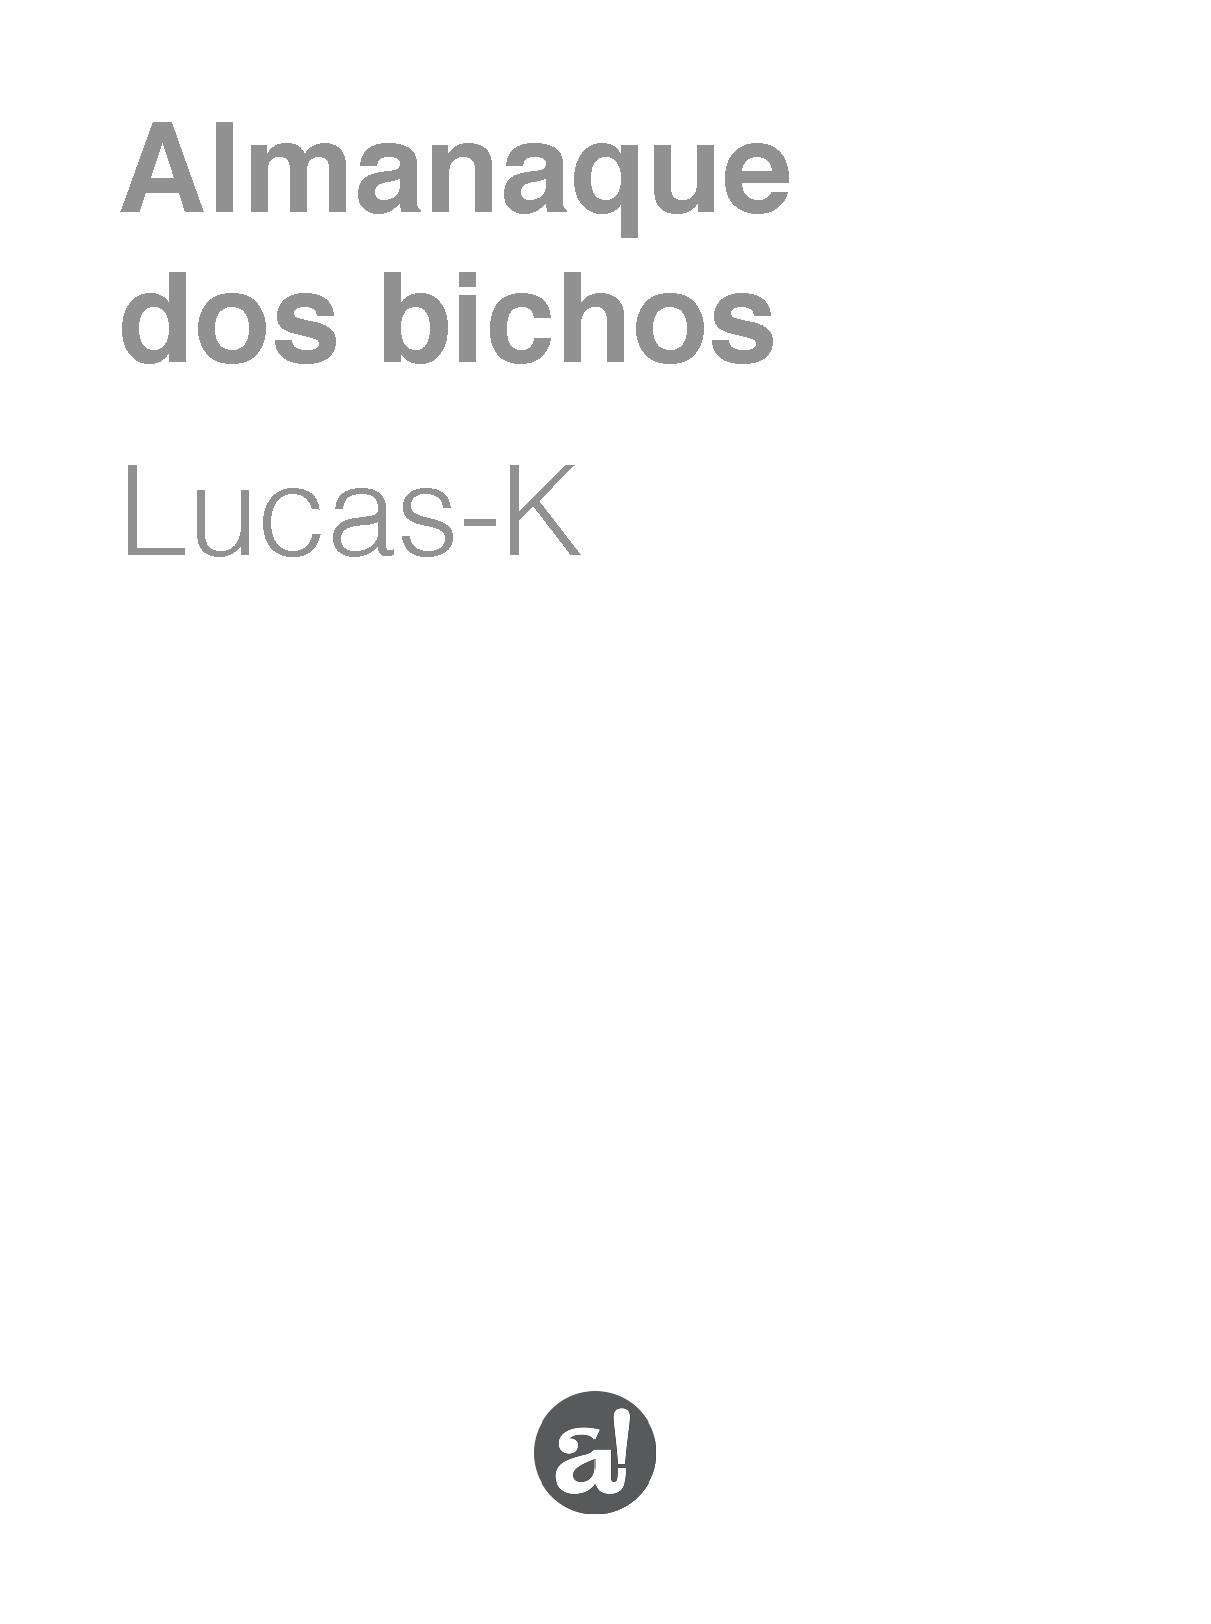
\includepdf[nup=2x2,                  % grid
            % offset=-15mm -5mm,        % posição
            % scale=.8,                 % tamanho da página
            % delta=4mm 4mm,            
            % frame,
            % pages={1-4}]{pdfs/PNLD2022-022_MIOLO.pdf}

\end{document}
